\chapter{Experimental Testbed for the Performance Evaluation}
\label{sec:tb}

The specifications of the systems used for our performance analysis are described
in Table~\ref{tab:hw}. 
%
The machines with Intel processors are based on the Ivy Bridge (IVB), Haswell
(HSW-D and HSW-S), Broadwell (BDW), Skylake (SKX), and Knights Landing (KNL)
microarchitectures. 
The first four microarchitectures are successors to each other and can be seen
as traditional superscalar, multicore, SIMD capable processors.
HSW-D and HSW-S are desktop and server systems, respectively.
The HSW-S systems has cluster-on-die (CoD) enabled. 
Here, the processor's local L3 cache is divided into two parts and the memory
forms two NUMA locality domains.
%
SKX is the server variant of the Skylake microarchitecture including support for
AVX-512 and hosts an additional FMA unit.
%
The Knights Landing processor is
%, in contrast to the previously mentioned processors, 
a representative of Intels Xeon Phi line, a manycore
architecture with SIMD lanes wider than in the formerly named processors.
It is the successor of the Knights Corner manycore processor.

The exact AVX-512 ISA (instruction set architecture) for Knights Lading differs from the Skylake incarnation,
but for our purpose is not relevant. 
Knights Lading includes a $16$\,GB large high bandwidth memory (HBM) with
bandwidths up to $450$\,GB/s; see also the discussion in section~\ref{sec:pa}.
We operate KNL in the flat memory model, where the DDR memory and HBM 
represent a NUMA domain, each.
%
AMD-based systems include a desktop (ZEN-D) and server (ZEN-S) system based on the Zen
microarchitecture. 
ZEN-S' processor with $24$ cores consists of four NUMA LDs.
%

The CPU frequencies on all machines were fixed to the base frequencies specified
in Table~\ref{tab:hw}.
On the ZEN systems we set the frequency to the nominal base frequency, but could
not disable AMD's turbo mode, which allows cores to run above this frequency.
For Knights Landing, altering frequencies are not supported and are handled by the
processor itself.
%
Furthermore, each thread's affinity was explicitly set.
%
For all arrays, large $2$~MiB pages were used.
%1 This was achieved by using transparent huge pages
%1 \footnote{\texttt{/sys/kernel/mm/transparent\_hugepage/[enabled|defrag]} were set to
%1 \texttt{always}.} as well as calling \texttt{madvise(MADV\_HUGEPAGE)} after
%1 allocation of memory.
%
First-touch policy was in place, and we verified via the NUMA-API that the data
always reside in the cores associated NUMA domain.
%
On all systems supporting simultaneous multithreading (SMT) only physical cores were used.
%
As compiler, Intel C/Fortran Compiler version 17.0.1 was used.

\section{Read-only memory bandwidth and machine balance}
\label{sec:tb:membw}

\begin{figure}[!t]%
  \centering%
  \captionsetup[subfigure]{farskip=0pt}%
  \subfloat[]{%
    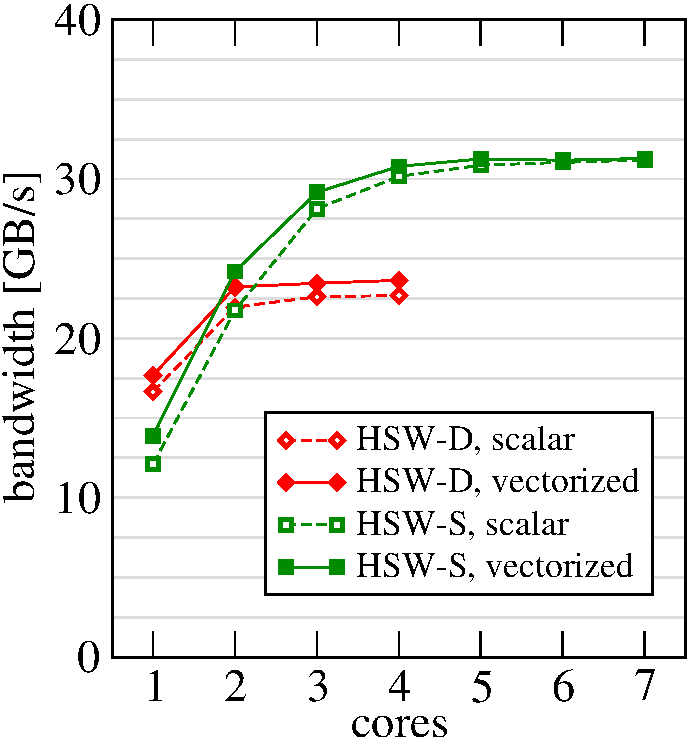
\includegraphics[height=0.4\linewidth,clip=true]{images/stream/StreamReadHswScalarVectorized}
    \label{fig:mrm:bw-scaling}
  } \, \hspace{0.5cm}
  \subfloat[]{%
    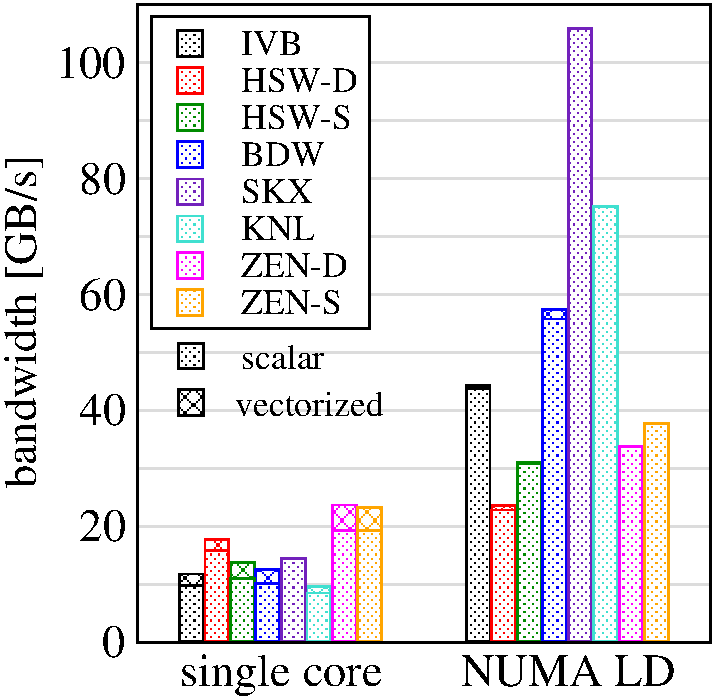
\includegraphics[height=0.4\linewidth,clip=true]{images/stream/StreamReadSingleCoreFullProcessor}
    \label{fig:mrm:bw-single-core}
  }%
  \caption{Bandwidth over the number of cores of the read only benchmark in a
scalar and vectorized version exemplified on HSW-D and
HSW-S~\protect\subref{fig:mrm:bw-scaling}.
Single core bandwidth and saturated bandwidth with all available cores of the
processor/cluster~\protect\subref{fig:mrm:bw-single-core}.}
  \label{fig:mrm:bw}
\end{figure}

The measured read-only bandwidth, required for the performance model, is
reported in Table~\ref{tab:hw}.
As discussed in section~\ref{sec:mrm} only scalar loads are used.
%
If enough cores are used then scalar and vectorized read-only benchmarks
saturate the memory bandwidth with the only difference being that the saturation of
the latter is already achieved with fewer cores. 
This is exemplified on HSW-D and HSW-S systems shown in
Figure~\ref{fig:mrm:bw-scaling}.
HSW-D and HSW-S show the typical saturation behavior for (current Intel) desktop
and server systems. 
Typically desktop systems nearly saturate the memory bandwidth with one core.
%
Figure~\ref{fig:mrm:bw-single-core} shows the difference between the scalar and
vectorized read-only benchmark for the single core and the usage of all cores
inside a NUMA LD over all systems in the test bed.
IVB, HSW-S, and the ZEN-based
systems reach,
with one core and vector loads between $15$\,\% and
$25$\,\%,
a higher bandwidth
than with scalar load instructions.
However, utilizing the full NUMA LD nearly no difference is visible.
%

% \section{Machine Balance $B_m$}
The machine balance $B_m$ from Table~\ref{tab:hw} considers the scalar read-only
memory bandwidths and the scalar double precision floating point capabilities of
the processors. 
This is either a scalar FMA or, if unavailable, a scalar addition and
multiplication for processing a nonzero.

%
% The code balance for sparse solve from from Tab.~\ref{tab:mrm:bc} when data
% resides in memory has in the best case its lowest value of $B_c = 4$\,B/F.
% This exceeds the machine balances of all systems in the test bed.
% According to the Roofline model, this indicates sparse solve is memory bound.

% The bandwidth between each cache level also shown in Table~\ref{tab:hw} is
% obtained from~\ref{intel-orm-2016}. 
% Despite the documentation reports $1$\,cy/cl between L1- and L2-cache for the
% Haswell microarchitecture, only around  half the bandwidth is observed to be
% reached~\cite{hofmann-2016-hsw}.
% Hence, we assume $2$\,cy/cl as bandwidth.
% vec faster than scalar in percent: (bw_vec / bw_scalar - 1) * 100
% ivb_emmy
% ["23.74"]
% bdw_broadep2
% ["17.94"]
% bdw_meggie
% ["7.78"]
% hsw_hasep1
% ["14.56"]
% knl_knightmare1
% ["12.64"]
% zen_summitridge1
% ["22.90"]
% zen_naples1
% ["20.44"]
% hsw_woody_hsw
% ["6.18"]
% sx_sxace
% ["0.00"]
% sks_skylakesp2
% ["-3.21"]


\section{Matrices}

% \begin{SCtable}[][t]
% %\begin{table}[tp]
%   \centering
%   \small
%   \begin{tabular}{ll|rrrrrr}
%   \hline
%          &&  \multicolumn{1}{c}{$\bm{n}$} &&
%             \multicolumn{1}{c}{$\bm{\text{nnz}(A)}$}  &&
%             \multicolumn{1}{c}{$\bm{\text{nnz}(L)}$}   \\ 
%   \hline
% % values for threads = 1, p = 80
%   dense  && $    20 \times 10^3$ && $200 \times 10^6$ &&  $  200 \times 10^6$  \\ % ps-n-20000-t-1-p-80
%   lapl1  && $   256 \times 10^3$ && $  3 \times 10^6$ &&  $  219 \times 10^6$  \\ % pl-n-40-b-4-t-1-p-80  N=40, B=4
%   lapl2  && $   343 \times 10^3$ && $  1 \times 10^6$ &&  $  166 \times 10^6$  \\ % pl-n-70-b-1-t-1-p-80  N=70, B=1
%   omen1  && $1\,751 \times 10^3$ && $ 32 \times 10^6$ && $1\,076 \times 10^6$  \\ % omen-rc2.5-lc160-t-1-p-80
%   omen2  && $   760 \times 10^3$ && $ 20 \times 10^6$ && $   690 \times 10^6$  \\ % omen-rc3.5-t-1-p-80
%   omen3  && $1\,271 \times 10^3$ && $ 42 \times 10^6$ && $1\,651 \times 10^6$  \\ % omen-rc4.5-t-1-p-80
%   bddc   && $   750 \times 10^3$ && $ 31 \times 10^6$ && $1\,590 \times 10^6$  \\ % mat\_Kii\_sd22\_size750141\_load2\_newton1
%   \hline
%   \end{tabular}
%   \caption{Dimension ($n$) and number of nonzeros ($\text{nnz}$) for $A$ and 
% $L$ for all benchmark matrices.}
%   \label{tab:m:list}
% % \end{table}
% \end{SCtable}


%In~Table~\ref{tab:m:list}, we present information on  
%the symmetric matrices which will be used
%for the performance modeling and experiments in the following sections.
Table~\ref{tab:m:list} lists matrix dimension ($n$), number of nonzeros in the
matrix ($\text{nnz}(A)$), and the factor (nnz$(L)$) of the matrices used for
benchmarking in the following sections.
% and the number of nonzeros in the factor ($\text{nnz}(L)$).
% It shows the matrix dimension ($n$), the number of nonzeros in the matrix ($\text{nnz}(A)$),  
% and the number of nonzeros in the factor ($\text{nnz}(L)$).
The reported numbers of nonzeros 
are reported for factorizations using single threaded execution
and a panel size $\panelsize = 80$. 
All matrices are sparse except 
for the first matrix \mymat{dense}, where both the matrix and  
the factor $L$ are dense. 
We use this dense matrix as a best case example for our single core performance
investigations.
The matrices \mymat{lapl1} and \mymat{lapl2} are test matrices arising from a
finite difference discretization of the Laplace operator in three dimensions
with Dirichlet boundary conditions. 
In addition, the matrix \mymat{lapl2} contains a block structure
of size $4$. 
The \mymat{omen} matrices correspond to a set of representative matrices from 
an atomistic nanoelectronic device engineering simulation code (\cite{luisier2011atomistic}).
The matrix \mymat{bddc} arises from a finite element discretization of a typical
solid mechanics problem. Here, as a material model, a J2-elasto-plasticity model
was chosen and three-dimensional and piecewise quadratic tetrahedral finite
elements were used for the discretization. The matrix \mymat{bddc} represents a
typical subdomain problem arising in the BDDC (Balancing Domain Decomposition by
constraints) implicit finite element solver.

% \sout{Matrix \uwave{\mymat{bddc1}}
% \mycomment{OR: gemeint ist wohl BDDC; sollte doch mehr Information dazu hinein?
% FETI stimmt nicht, Referenz stimmt nicht}
% has been obtained from 
% \uwave{a finite element tearing and interconnecting (FETI)} code~\cite{klawonn2002dual}.
% Figure~\ref{fig:m:spy} shows the structure of $A$ for the different matrix
% classes.}
%, whereas more  interesting, is the nonzero distribution over the panel sizes of the factor $L$ found in 
%Figure~\ref{fig:m}.

Please note that the current factorization limits the number of parts to powers
of two.
To avoid load imbalance during the solve step we report results only for thread
counts which are powers of two.
%
%This leads to a load imbalance during the solve step, which is why in this
%article we only report results for thread counts which are equal to powers of
%two.

\begin{figure}[tp]
  \centering
  \captionsetup[subfigure]{farskip=0pt}%
  \subfloat[lapl]{%
    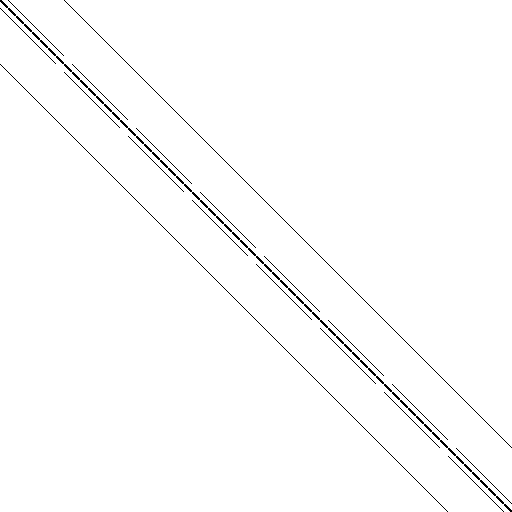
\includegraphics[width=0.25\linewidth,clip=true]{images/spy-plots/a-pl-n-8-b-1}
    \label{fig:m:spy:lp}
  }\,
  \subfloat[omen]{%
    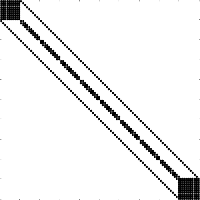
\includegraphics[width=0.25\linewidth,clip=true]{images/spy-plots/omen}
    \label{fig:m:spy:omen}
  }\,
  \subfloat[bddc]{%
    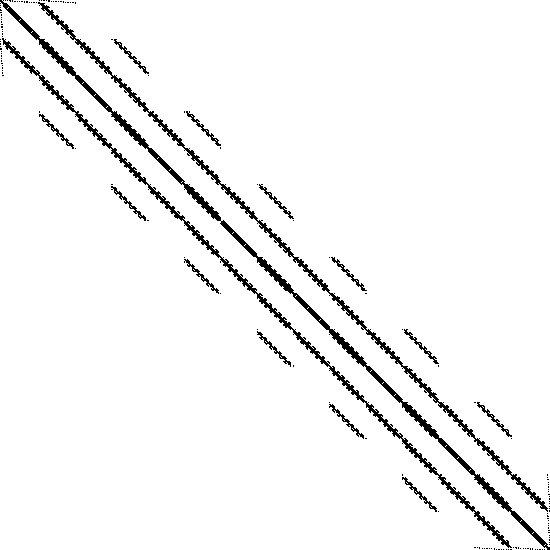
\includegraphics[width=0.25\linewidth,clip=true]{images/spy-plots/mat_Kii_sd89_size10992_load2_newton1}
    \label{fig:m:spy:feti}
  } 
  \caption{Structure of $A$ for matrix classes lapl~\protect\subref{fig:m:spy:lp},
  omen~\protect\subref{fig:m:spy:omen}, and bddc~\protect\subref{fig:m:spy:feti}.}
  \label{fig:m:spy}
\end{figure}

% {{{
% To generate/alter images:
% - go to directory data/matrices
%
% - run: ./plot-log.py <matrix-name>.dat
%   this will generate a pdf and png of the histogram.
%
% - copy the pdf to images/matrices
%
% \begin{figure*}[tp]
%   \centering
%   \subfloat[dense]{%
%     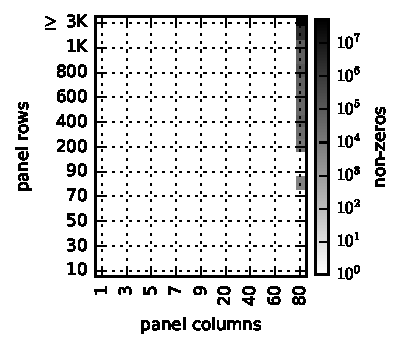
\includegraphics[width=0.3\textwidth,clip=true]{images/matrices/ps-n-20000-t-1-p-80}
%     \label{fig:m:dense}
%   } \,
%   \subfloat[lapl1]{%
%     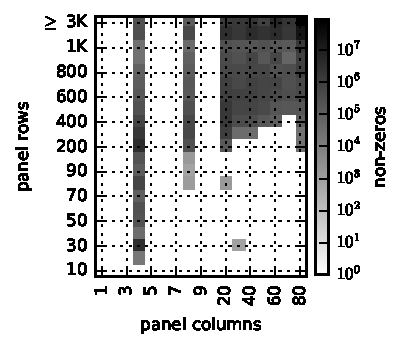
\includegraphics[width=0.3\textwidth,clip=true]{images/matrices/pl-n-00040-b-004}
%     \label{fig:m:laplace:n40b4}
%   } \,
%   \subfloat[lapl2]{%
%     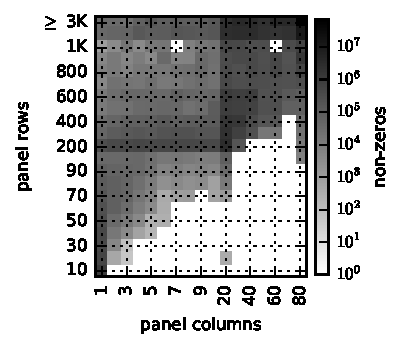
\includegraphics[width=0.3\textwidth,clip=true]{images/matrices/pl-n-70-b-1-t-1-p-80}
%     \label{fig:m:laplace:n70b1}
%   } \,
%   \subfloat[omen1]{%
%     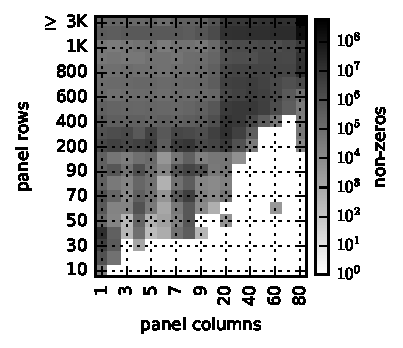
\includegraphics[width=0.3\textwidth,clip=true]{{{images/matrices/omen-rgf-tc2.5-lc160-t-1-p-80.hist-rhs-update-frequencies}}}
%     \label{fig:m:omen}
%   } \,
%   \subfloat[omen2]{%
%     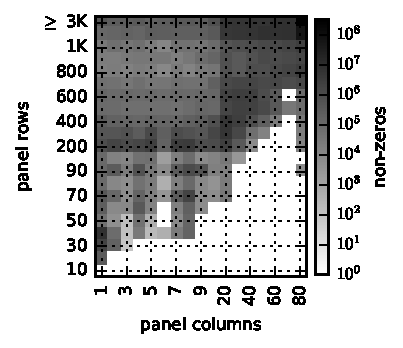
\includegraphics[width=0.3\textwidth,clip=true]{{{images/matrices/omen-rgf-tc3.5-t-1-p-80.hist-rhs-update-frequencies}}}
%     \label{fig:m:omen}
%   } \,
% %  \subfloat[omen3]{%
% %    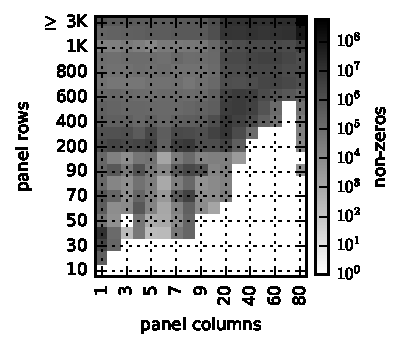
\includegraphics[width=0.3\textwidth,clip=true]{{{images/matrices/omen-rgf-tc4.5-t-1-p-80.hist-rhs-update-frequencies}}}
% %    \label{fig:m:omen}
% %  } \,
%   \subfloat[feti1]{%
%     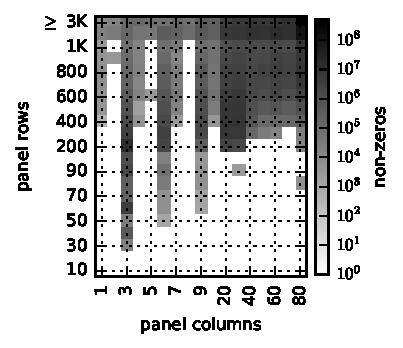
\includegraphics[width=0.3\textwidth,clip=true]{{{images/matrices/mat_Kii_sd22_size750141_load2_newton1-t-1-p-80.log-rhs-update-frequencies}}}
%     \label{fig:m:omen}
%   } \,
%   \caption{Multi-parameter histograms showing how many nonzeros of $L$ are in panels with a certain
%            number of columns and rows. Panels with $3000$ and more rows are
%            accumulated.
%            This plot gives an impression of how the work, i.e.,\ nonzeros,
%            in~$L$ is distributed over panel dimensions.
%   }
%   \label{fig:m}
% \end{figure*}
% }}}